\documentclass[11pt, twoside, pdftex]{article}

% This include all the settings that we should use for the document
\newcommand{\PDFTitle}{Using the ARM* Generic Interrupt Controller}
\newcommand{\commonPath}{../../Common}
\newcommand{\datePublished}{Mar 2022}

\newcommand{\versnum}{21.1} %version number quartus/AMP
\newcommand{\quartusname}{Quartus\textsuperscript{\textregistered} Prime}	
\newcommand{\textBar}{For \quartusname{} \versnum{}}
\newcommand{\thisyear}{2022 } %for copyright
\newcommand{\company}{FPGAcademy.org}
\newcommand{\longteamname}{FPGAcademy.org}
\newcommand{\teamname}{FPGAcademy}
\newcommand{\website}{FPGAcademy.org}

\newcommand{\productAcronym}{AMP}
\newcommand{\productNameShort}{Monitor Program}

\newcommand{\productNameMedTM}{Monitor Program}
\newcommand{\productNameMed}{Monitor Program}

%\newcommand{\headerLogoFilePath}[1]{#1/FPGAcademy.png}



\setlength\topmargin{-0.25in}
\setlength\headheight{0in}
\setlength\headsep{0.35in}
\setlength\textheight{8.5in}
\setlength\textwidth{7in}
\setlength\oddsidemargin{-0.25in}
\setlength\evensidemargin{-0.25in}
\setlength\parindent{0.25in}
\setlength\parskip{0in} 

\pdfpagewidth 8.5in
\pdfpageheight 11in

% listings is a package that supports encapsulating source code in LaTeX conveniently

\usepackage{listings}
% add support for graphics
\usepackage{graphicx}
\usepackage[usenames, dvipsnames]{color}

\def\expandparam\lstinputlisting[#1]#2{\edef\tmp{\noexpand\lstinputlisting[#1]{#2}}\tmp}

\widowpenalty 10000
\clubpenalty 10000

%%%%%%%%%%%%%%%%%%%% Source Code Formatting %%%%%%%%%%%%%%%%%%%%
\definecolor{globalCommentColour}{rgb}{0.588,0.588,0.588}

%%%%%%%%%%%%%%%%%%%%%%%%%%%%%%%%%%%%%%%%%%%%%%%%%%%%
% Defining a NiosII ASM highlighter for lstlisting
\lstdefinelanguage[NiosII]{Assembler} {
 	morekeywords={add, addi, and, andhi, andi, beq, bge, bgeu, bgt, bgtu, ble,  bleu, blt, bltu, bne, br, break,% 
 	bret, call, callr, cmpeq, cmpeqi, cmpge, cmpgei, cmpgeu, cmpgeui, cmpgt, cmpgti, cmpgtu, cmpgtui, cmple,%
 	cmplei, cmpleu, cmpleui, cmplt, cmplti, cmpltu, cmpltui, cmpne, cmpnei, custom, div, divu, eret, flushd,%
 	flushda, flushi, flushp, initd, initda, initi, jmp, jmpi, ldb, ldbio, ldbu, ldbuio, ldh, ldhio, ldhu, ldhuio,%
 	ldw, ldwio, mov, movhi, movi, movia, movui, mul, muli, mulxss, mulxsu, mulxuu, nextpc, nop, nor, or, orhi, ori,%
 	rdctl, rdprs, ret, rol, roli, ror, sll, slli, sra, srai, srl, srli, stb, stbio, sth, sthio, stw, stwio,%
 	sub, subi, sync, trap, wrctl, wrtcl, wrprs, xor, xori, xorhi, xori},% 	
 	morekeywords=[2]{.abort, .ABORT, .align, .app-file, .ascii, .asciz, .balign, .byte, .comm, .data, .def,%
 	.desc, .dim, .double, .eject, .else, .end, .endef, .endif, .equ, .equiv, .err, .extern, .file, .fill, .float,%
 	.global, .globl, .hword, .ident, .if, .include, .int, .irp, .irpc, .lcomm, .lflags, .line, .linkonce, .ln,%
 	.list, .long, .macro, .mri, .nolist, .octa, .org, .p2align, .psize, .quad, .rept, .sbttl, .scl, .section,%
 	.set, .short, .single, .size, .sleb128, .skip, .space, .stadb, .stabn, .stabs, .string, .symver, .tag,%
 	.text, .title, .type, .val, .uleb128, .word},% 	
 	morekeywords=[3]{et, bt, gp, sp, fp, ea, sstatus, ra, pc, status, estatus, bstatus, ienable, ipending, cpuid,%
 	exception, pteaddr, tlbacc, tlbmisc, eccinj, badaddr, config, mpubase, mpuacc},% 	
 	sensitive=t,%
 	alsoletter=.,%
	morestring=[b]",%
 	morecomment=[s]{/*}{*/},%
 	morecomment=[l]\#,%
   }[keywords,comments,strings]
   
   %% NOTE: morekeywords=[2] are GNU directives.
   
   \definecolor{niosInstructionColour}{rgb}{0.000,0.608,0.000}
   \definecolor{niosDirectiveColour}{rgb}{0.000,0.000,0.902}
   \definecolor{niosSpecialRegColour}{rgb}{0.000,0.000,0.000}
   \definecolor{niosStringColour}{rgb}{0.808,0.482,0.000}
   
   %% NOTE: To make bold use: =\bfseries\color{<colour>}
   \lstdefinestyle{defaultNiosStyle} {
   language=[NiosII]{Assembler},
   stringstyle=\color{niosStringColour},
   keywordstyle=\color{niosInstructionColour},
   keywordstyle=[2]\color{niosDirectiveColour},
   keywordstyle=[3]\itshape\color{niosSpecialRegColour}
   }
%%%%%%%%%%%%%%%%%%%%%%%%%%%%%%%%%%%%%%%%%%%%%%%%%%%%

%%%%%%%%%%%%%%%%%%%%%%%%%%%%%%%%%%%%%%%%%%%%%%%%%%%%
% Defining a ArmA9 ASM highlighter for lstlisting
\lstdefinelanguage[ArmA9]{Assembler} {
 	morekeywords={ADC, ADD, ADDS, AND, ANDS, B, BAL, BEQ, BGE, BGT, BL, BLT, BIC, BKPT, BLX, BNE, BX, CDP, CLZ, CMN, CMP, EOR,%
 	EORS, LDC, LDM, LDR, LDRB, LDRBT, LDRH, LDRSB, LDRSH, LDRT, LSL, MCR, MLA, MOV, MOVW, MOVT, MRC, MRS, MSR, MUL, MVN, ORR, PLD,%
 	ROR, RSB, RSC, SBC, SMLAL, SMULL, STC, STM, STR, STRB, STRBT, STRH, STRT, SUB, SUBS, SWI, SWP, SWPB, TEQ, UMLAL,
 	PUSH, POP, MOVS, RORS, LSR},%
 	morekeywords=[2]{.abort, .ABORT, .align, .app-file, .ascii, .asciz, .balign, .byte, .comm, .data, .def,%
 	.desc, .dim, .double, .eject, .else, .end, .endef, .endif, .equ, .equiv, .err, .extern, .file, .fill, .float,%
 	.global, .globl, .hword, .ident, .if, .include, .int, .irp, .irpc, .lcomm, .lflags, .line, .linkonce, .ln,%
 	.list, .long, .macro, .mri, .nolist, .octa, .org, .p2align, .psize, .quad, .rept, .sbttl, .scl, .section,%
 	.set, .short, .single, .size, .sleb128, .skip, .space, .stadb, .stabn, .stabs, .string, .symver, .tag,%
 	.text, .title, .type, .val, .vectors, .uleb128, .word},%
 	morekeywords=[3]{SP, PC, MIDR, CTR, TCMTR, TLBTR, MPIDR, ID_PFR0, ID_PFR1, ID_DFR0, ID_MMFR0, ID_MMFR1, ID_MMFR2,%
 	ID_MMFR3, ID_ISAR0, ID_ISAR1, ID_ISAR2, ID_ISAR3, ID_ISAR4, CCSIDR, CLIDR, AIDR, CSSELR, TTBR0, TTRB1, TTBR2, DACR,%
 	DFSR, IFSR, ADFSR, AIFSR, DFAAR, IFAR, ICIALLUIS, BPIALLIS, PAR, ICIALLU, ICIMVAU, BPIALL, DCIMVAC, DCISW, V2PCWPR,%
 	DCCVAC, DCCSW, DDIMVAC, DCISW, TLBALLIS, TLBIMVAIS, TLBIASIDIS, TLBIMVAAIS, TLBIALL, TLBIMVA, TLBIASID, TLBIMVAA,%
 	PMCR, PMCNTENSET, PMCNTENCLR, PMOVSR, PMSWINC, PMSELR, PMXEVTYPER, PMXEVCNTR, PMUSERENR, PMINTENSET, PMINTENCLR,%
 	PRRR, NRRR, PLEIDR, PLEASR, PLEFSR, PLEUAR, PLEPCR, VBAR, MVBAR, ISR, FCSEIDR, CONTEXTIDR, TPIDRURW, TPIDRURO, TPIDRPRW},%
 	sensitive=f,%
 	alsoletter=.,%
	morestring=[b]",%
 	morecomment=[s]{/*}{*/},%
 	morecomment=[l]{//},%
   }[keywords,comments,strings]
   
   %% NOTE: morekeywords=[2] are GNU directives.
   
   \definecolor{armInstructionColour}{rgb}{0.000,0.608,0.000}
   \definecolor{armDirectiveColour}{rgb}{0.000,0.000,0.902}
   \definecolor{armSpecialRegColour}{rgb}{0.000,0.000,0.000}
   \definecolor{armStringColour}{rgb}{0.808,0.482,0.000}
   
   \lstdefinestyle{defaultArmStyle} {
   language=[ArmA9]{Assembler},
   stringstyle=\color{armStringColour},
   keywordstyle=\color{armInstructionColour},
   keywordstyle=[2]\color{armDirectiveColour},
   keywordstyle=[3]\itshape\color{armSpecialRegColour}
   }
%%%%%%%%%%%%%%%%%%%%%%%%%%%%%%%%%%%%%%%%%%%%%%%%%%%%

%%%%%%%%%%%%%%%%%%%%%%%%%%%%%%%%%%%%%%%%%%%%%%%%%%%%
% Defining style for the verilog.

\definecolor{verilogCommentColour}{rgb}{0.000,0.502,0.000}

\lstdefinestyle{defaultVerilogStyle} {
language={Verilog},
keywordstyle=\color{blue},
commentstyle=\color{verilogCommentColour}
}
%%%%%%%%%%%%%%%%%%%%%%%%%%%%%%%%%%%%%%%%%%%%%%%%%%%%

%%%%%%%%%%%%%%%%%%%%%%%%%%%%%%%%%%%%%%%%%%%%%%%%%%%%
% Defining style for the vhdl.
\lstdefinestyle{defaultVHDLStyle} {
language={VHDL},
keywordstyle=\color{blue},
commentstyle=\color{verilogCommentColour}
}
%%%%%%%%%%%%%%%%%%%%%%%%%%%%%%%%%%%%%%%%%%%%%%%%%%%%

%%%%%%%%%%%%%%%%%%%%%%%%%%%%%%%%%%%%%%%%%%%%%%%%%%%%
% Java
\definecolor{javaStringColour}{rgb}{0.808,0.482,0}
%%%%%%%%%%%%%%%%%%%%%%%%%%%%%%%%%%%%%%%%%%%%%%%%%%%%

%%%%%%%%%%%%%%%%%%%%%%%%%%%%%%%%%%%%%%%%%%%%%%%%%%%%
% Defining language styles
% C
\definecolor{CStringColour}{rgb}{0.808,0.482,0}
%%%%%%%%%%%%%%%%%%%%%%%%%%%%%%%%%%%%%%%%%%%%%%%%%%%%

%%%%%%%%%%%%%%%%%%%%%%%%%%%%%%%%%%%%%%%%%%%%%%%%%%%%
% Defining extended LaTeX language.
\lstdefinelanguage[LocalLaTeX]{TeX}[LaTeX]{TeX}%
 	{moretexcs={bf, it, sf, lstset},%
   	}%

\lstdefinestyle{defaultLocalLatexStyle} {
language=[LocalLatex]{TeX},
keywordstyle=\color{blue}\bfseries,
keywordstyle=[2]\color{blue},
keywordstyle=[3]\color{blue}\bfseries
}
%%%%%%%%%%%%%%%%%%%%%%%%%%%%%%%%%%%%%%%%%%%%%%%%%%%%

\lstset{
%language = C,
%language = Verilog,
%basicstyle=\color{black}\rmfamily\ttfamily,
basicstyle=\small\color{black}\ttfamily,
commentstyle=\small\color{globalCommentColour}\itshape\ttfamily,
keywordstyle=\small\color{blue}\bfseries\ttfamily,
showstringspaces=false,
frame=none, %lines % boxed listings
breaklines=true,
breakatwhitespace=true,
tabsize=4
}
%%%%%%%%%%%%%%%%%%%%%%%%%%%%%%%%%%%%%%%%%%%%%%%%%%%%%%%%%%%%%%%%


%\usepackage[centering]{geometry}.
%%%%%%%%%%%%%%%%%%%%%%%%%%%%%%%%%%%%%%%%%%%%%%%%%%%
% Document Settings
\usepackage[labelsep=period]{caption}
% we can choose a better font later
%\usepackage{palatino}
\usepackage{fourier}
%\fontencoding{T1}
% include common used symbols
\usepackage{textcomp}
% add support for graphics
\usepackage{graphicx}
\usepackage[usenames, dvipsnames]{color}
% enable to draw thick or thin table hlines
\setlength{\doublerulesep}{\arrayrulewidth}
\usepackage{longtable}
\setlongtables
%\usepackage{array}
% It may be better to use PDFLaTeX as it can generate bookmarks for the
% document

% Add some useful packages
\usepackage{ae,aecompl}
\usepackage{epsfig,float,times}

% reset the font for section
\usepackage{sectsty}
%\allsectionsfont{\fontfamily{ptm}\selectfont}
\allsectionsfont{\usefont{OT1}{phv}{bc}{n}\selectfont}

% use compact space for sections
\usepackage[compact]{titlesec}
\titlespacing{\section}{0pt}{0.2in}{*0}
\titlespacing{\subsection}{0pt}{0.1in}{*0}
\titlespacing{\subsubsection}{0pt}{0.05in}{*0}

% fancyhdr header and footer customization
\usepackage{layout}
\usepackage{fancyhdr}
\pagestyle{fancy}
\fancyhead{}
\fancyhead[R]{\textit{\tiny{\textBar}}}
\fancyfoot{}
\fancyfoot[LO,
RE]{\textrm{\href{https://www.fpgacademy.org}{\small \longteamname}} \\ {\small \datePublished }}
\fancyfoot[RO, LE]{\small \thepage}
% two-side settings
%\fancyhead{} % clear all header fields
%\fancyfoot{} % clear all footer fields
%\fancyfoot[LE,RO]{\thepage}
\renewcommand{\headrulewidth}{2pt}
\renewcommand{\headrule}{{\color{blue} \hrule width\headwidth height\headrulewidth \vskip-\headrulewidth}}
\renewcommand{\footrulewidth}{0pt}

% Format the footer on page 1
\fancypagestyle{plain}{
\fancyhead{}
\fancyfoot{}
\fancyfoot[LO,
RE]{\textrm{\href{https://www.fpgacademy.org}{\small \longteamname}} \\ {\small \datePublished }}
\fancyfoot[RO, LE]{\small \thepage}
\renewcommand{\headrulewidth}{0pt}
}
% adjust some setting to try to make the figure stay in the same page with text
% Reference: 	http://www.cs.uu.nl/~piet/floats/node1.html
%   			http://mintaka.sdsu.edu/GF/bibliog/latex/floats.html
%   General parameters, for ALL pages:
\renewcommand{\topfraction}{0.9}	% max fraction of floats at top
\renewcommand{\bottomfraction}{0.8}	% max fraction of floats at bottom
%   Parameters for TEXT pages (not float pages):
\setcounter{topnumber}{3}
\setcounter{bottomnumber}{3}
\setcounter{totalnumber}{5}     % 2 may work better
\setcounter{dbltopnumber}{2}    % for 2-column pages
\renewcommand{\dbltopfraction}{0.9}	% fit big float above 2-col. text
\renewcommand{\textfraction}{0.07}	% allow minimal text w. figs
%   Parameters for FLOAT pages (not text pages):
\renewcommand{\floatpagefraction}{0.7}	% require fuller float pages
% N.B.: floatpagefraction MUST be less than topfraction !!
\renewcommand{\dblfloatpagefraction}{0.7}	% require fuller float pages
%%%%%%%%%%%%%%%%%%%%%%%%%%%%%%%%%%%%%%%%%%%%%%%%%%%
% remember to use [htp] or [htpb] for placement
%%%%%%%%%%%%%%%%%%%%%%%%%%%%%%%%%%%%%%%%%%%%%%%%%%%

% set no indent for paragraph
\setlength{\parindent}{0em}
\addtolength{\parskip}{11pt}
\newcommand{\compact}{[topsep=0pt]}
% use this package to reduce space
\usepackage{enumitem}
\usepackage{multirow}
\usepackage{rotating}
\usepackage{pifont}
\usepackage{dingbat}
\newcommand{\itemsecond}{$\circ$}
%
%%%%%%%%%%%%%%%%%%
\date{}
\author{}
%%%%%%%%%%%%%%%%%%
\newcommand{\de}{DE-series}
\newcommand{\up}{FPGAcademy}
\newcommand{\fabric}{Avalon Switch Fabric}
\newcommand{\TODO}[1]{\textcolor{red}{\textbf{TODO}: #1}}
\def\registered{{\ooalign{\hfil\raise .00ex\hbox{\scriptsize R}\hfil\crcr\mathhexbox20D}}}

% enable url and reference(bookmarks) in pdf
\usepackage{url}
\usepackage[pdftex, colorlinks]{hyperref}
\hypersetup{%
pdftitle={\PDFTitle},
linkcolor=blue,
hyperindex=true,
pdfauthor={\longteamname},
pdfkeywords={FPGAcademy, Academic Program, Example System},
bookmarksnumbered,
bookmarksopen=false,
filecolor=blue,
pdfstartview={FitH},
urlcolor=blue,
plainpages=false,
pdfpagelabels=true,
linkbordercolor={1 1 1} %no color for link border
}%
%%%%%%%%%%%%%%%%%%%%%%%%%%%%%%%%%%%%%%%%%%%%%%%%%%%
\setlength{\fboxsep}{0.7pt}
\setlength{\fboxrule}{0.5pt}

\newcommand{\red}[1]{{\color{red}\sf{#1}}}
\newcommand{\blue}[1]{{\color{blue}\sf{#1}}}



%%%%%%%%%%%%%%%%%%%%%%%%%
% Add title
\newcommand{\doctitle}{Using the ARM* \\ Generic Interrupt Controller}
\newcommand{\dochead}{Using the ARM* Generic Interrupt Controller}
% Usually no need to change these two lines
\title{\fontfamily{phv}\selectfont{\doctitle} }
\chead{ \small{\textsc{\bfseries \dochead} } }
% Customizations
%%%%%%%%%%%%%%%%%%%%%%%%%
% Allows multiple figures per page

\renewcommand\floatpagefraction{.9}
\renewcommand\topfraction{.9}
\renewcommand\bottomfraction{.9}
\renewcommand\textfraction{.1}   
\setcounter{totalnumber}{50}
\setcounter{topnumber}{50}
\setcounter{bottomnumber}{50}
\widowpenalty 10000
\clubpenalty 10000
\raggedbottom

%%%%%%%%%%%%%%%%%%
%%% DOCUMENT START
%\begin{document}
\begin{document}
\begin{table}
    \centering
    \begin{tabular}{p{5cm}p{4cm}}
        \hspace{-3cm}
        &
        \raisebox{1\height}{\parbox[h]{0.5\textwidth}{\Large\fontfamily{phv}\selectfont{\textsf{\doctitle}}}}
    \end{tabular}
    \label{tab:logo}
\end{table}

\colorbox[rgb]{0,0.384,0.816}{\parbox[h]{\textwidth}{\color{white}\textsf{\textit{\textBar}}}}

\thispagestyle{plain}
 
\section{Introduction}

This document introduces the ARM* Generic Interrupt Controller (GIC), which is included as
part of the ARM Cortex-A9* MPCORE* processor in the Intel\textsuperscript{\textregistered} Cyclone\textsuperscript{\textregistered} V SoC family. We do not discuss
some of the advanced features of the GIC in this document; complete information is available 
in the publication entitled {\it ARM Generic Interrupt Controller
Architectural Specification}, which is available from ARM Holdings. 
\\
\\
{\bf Contents}:
\begin{itemize}
\item Purpose of the GIC
\item ARM Exception Processing Architecture
\item GIC Architecture
\item GIC Programmer's Interface
\item Examples of ARM Software Code for the GIC
\end{itemize}
\clearpage
\newpage

\section{ARM* Generic Interrupt Controller}
As illustrated in Figure~\ref{fig:arm_MPCORE}, 
the ARM {\it generic interrupt controller} (GIC) is a part of the
ARM A9 MPCORE processor.  The GIC is connected to the IRQ interrupt signals of
all I/O peripheral devices that are capable of generating interrupts.  Most of these
devices are normally external to the A9 MPCORE, and some are internal peripherals (such as
timers). The GIC included
with the A9 MPCORE processor in the Intel Cyclone V SoC family handles up to 255 
sources of interrupts. When a peripheral device sends its IRQ signal to the GIC, then the
GIC can forward a corresponding IRQ signal to one or both of the A9 cores.
Software code that is running on the A9 core can then query the GIC to determine which 
peripheral device caused the interrupt, and take appropriate action. The procedure for 
working with interrupts for the ARM Cortex-A9 and the GIC are described in the following sections.
~\\
~\\
\begin{figure}[h!]
   \begin{center}
		 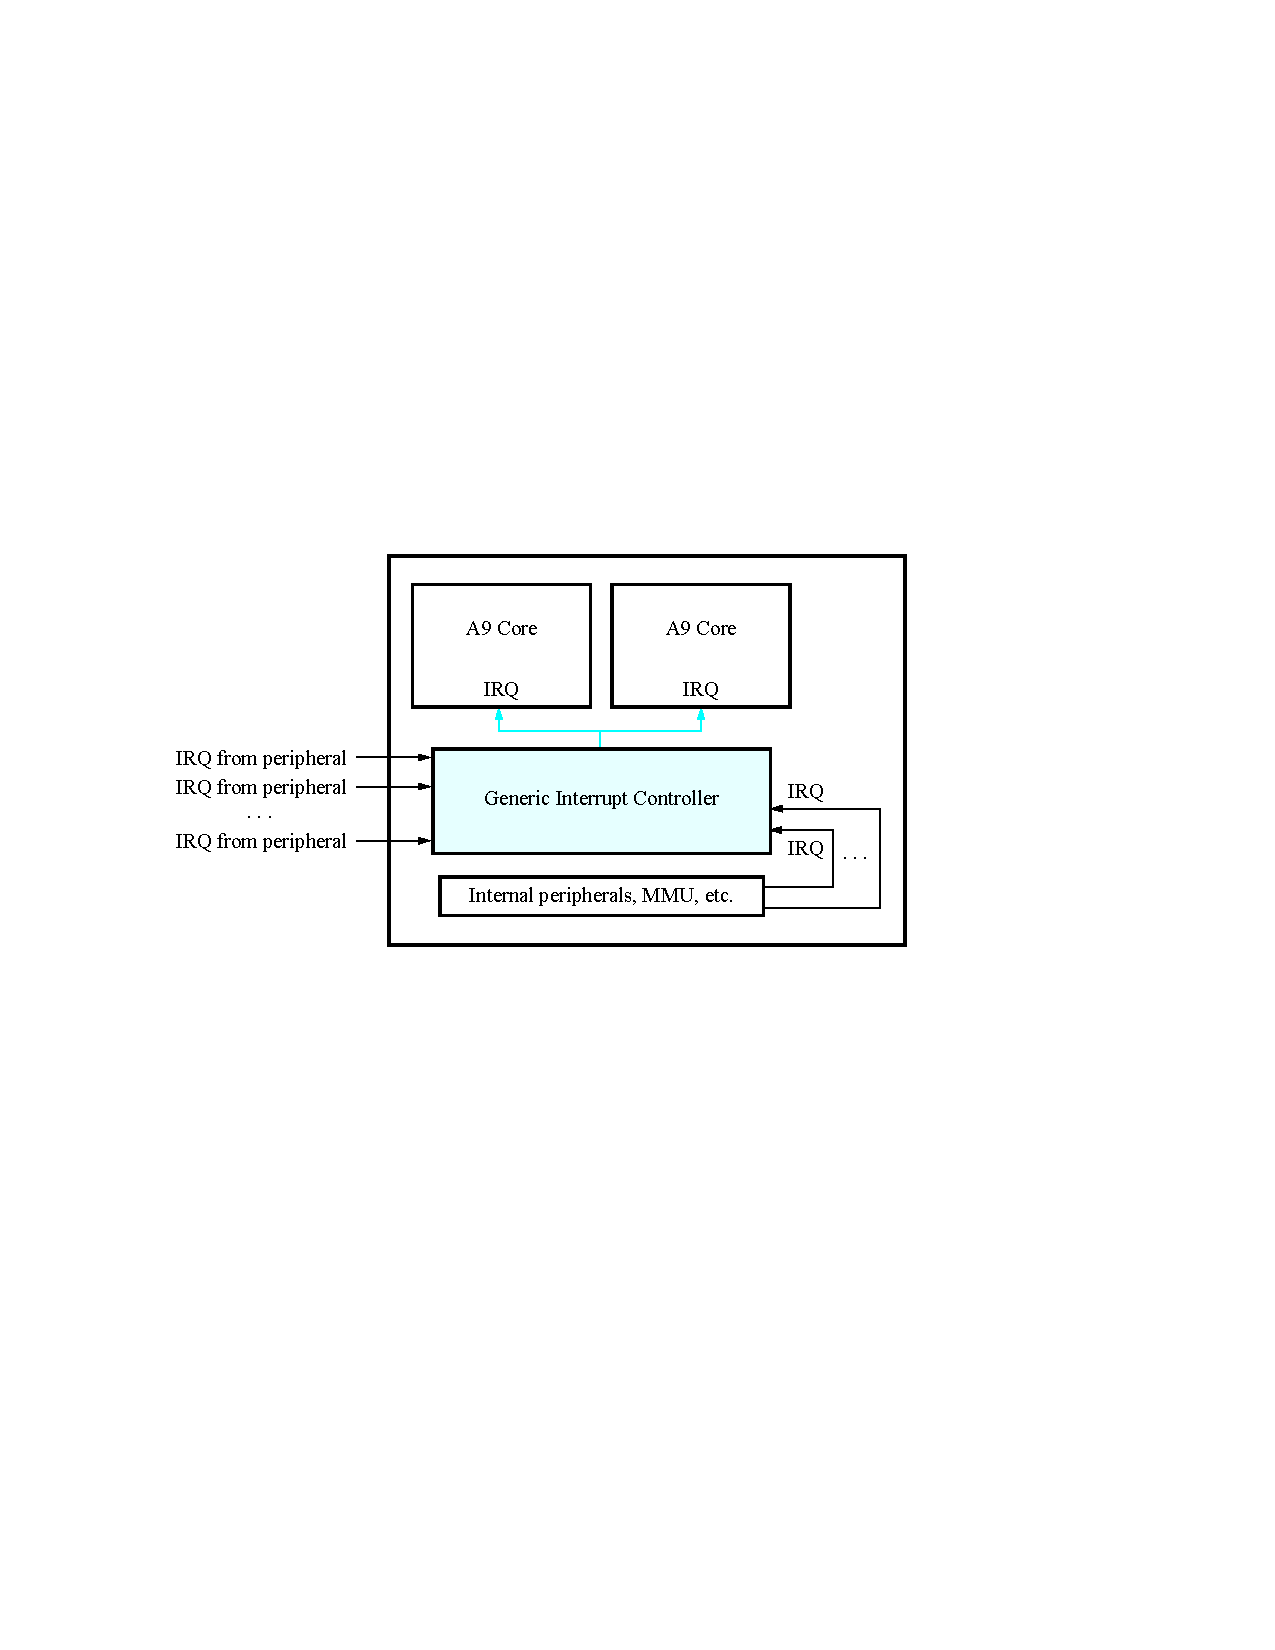
\includegraphics{figures/ARM_A9_GIC.pdf}
   \end{center}
   \caption{The ARM A9 MPCORE processor.}
	\label{fig:arm_MPCORE}
\end{figure}

\section{Interrupts in the ARM Cortex-A9*}
An introduction to ARM processors can be found in the tutorial {\it Introduction to the
ARM Processor Using Intel/ARM Toolchain},  which is available on Intel's FPGA University 
Program website.  As described in that tutorial, the ARM Cortex-A9 has several main modes of 
operation, listed below:
\begin{itemize}
\item {\it User} mode -- is the basic mode in which application
programs run. This is an unprivileged mode, which has restricted
access to system resources.
\item {\it System} mode -- provides full access to system
resources. It can be entered only from one of the exception
modes listed below.
\item {\it Supervisor} mode -- is entered when the processor executes
a {\it supervisor call} instruction, SVC. It is also entered on reset or power-up.
\item {\it Abort} mode -- is entered if the processor attempts to access a non-legitimate memory
		  location. This can happen, for example, when performing a word access for
		  an address that is not word-aligned.
\item {\it Undefined} mode -- is entered if the processor
attempts to execute an unimplemented instruction.
\item {\it IRQ} mode -- is entered in response to an interrupt request.
\item {\it FIQ} mode -- is entered in response to a {\it fast interrupt} request. We do not 
discuss fast interrupts in this document; they are used in some Cortex-A9 systems to 
provide faster service for more urgent requests. This document focuses only on IRQ interrupts.
\end{itemize}

When the processor is first powered on, or reset, it is in the {\it Supervisor}
mode. This mode is {\it privileged}, which means that it allows the use of all processor
instructions and operations. From supervisor mode it is possible to 
change into {\it User} mode, which is the only non-privileged mode. In User mode certain types
of processor operations and instructions are prohibited. In practice, the Supervisor mode is 
normally used when the processor is executing software such as an operating system,
whereas other software code may run in the User mode, thereby providing a level of protection 
for critical resources.

The operating mode of the processor is indicated in the current processor status register
CPSR, as depicted in Figure~\ref{fig:arm_cpsr}. The mode bits are defined in Table 1. 

\begin{figure}[h!]
   \begin{center}
       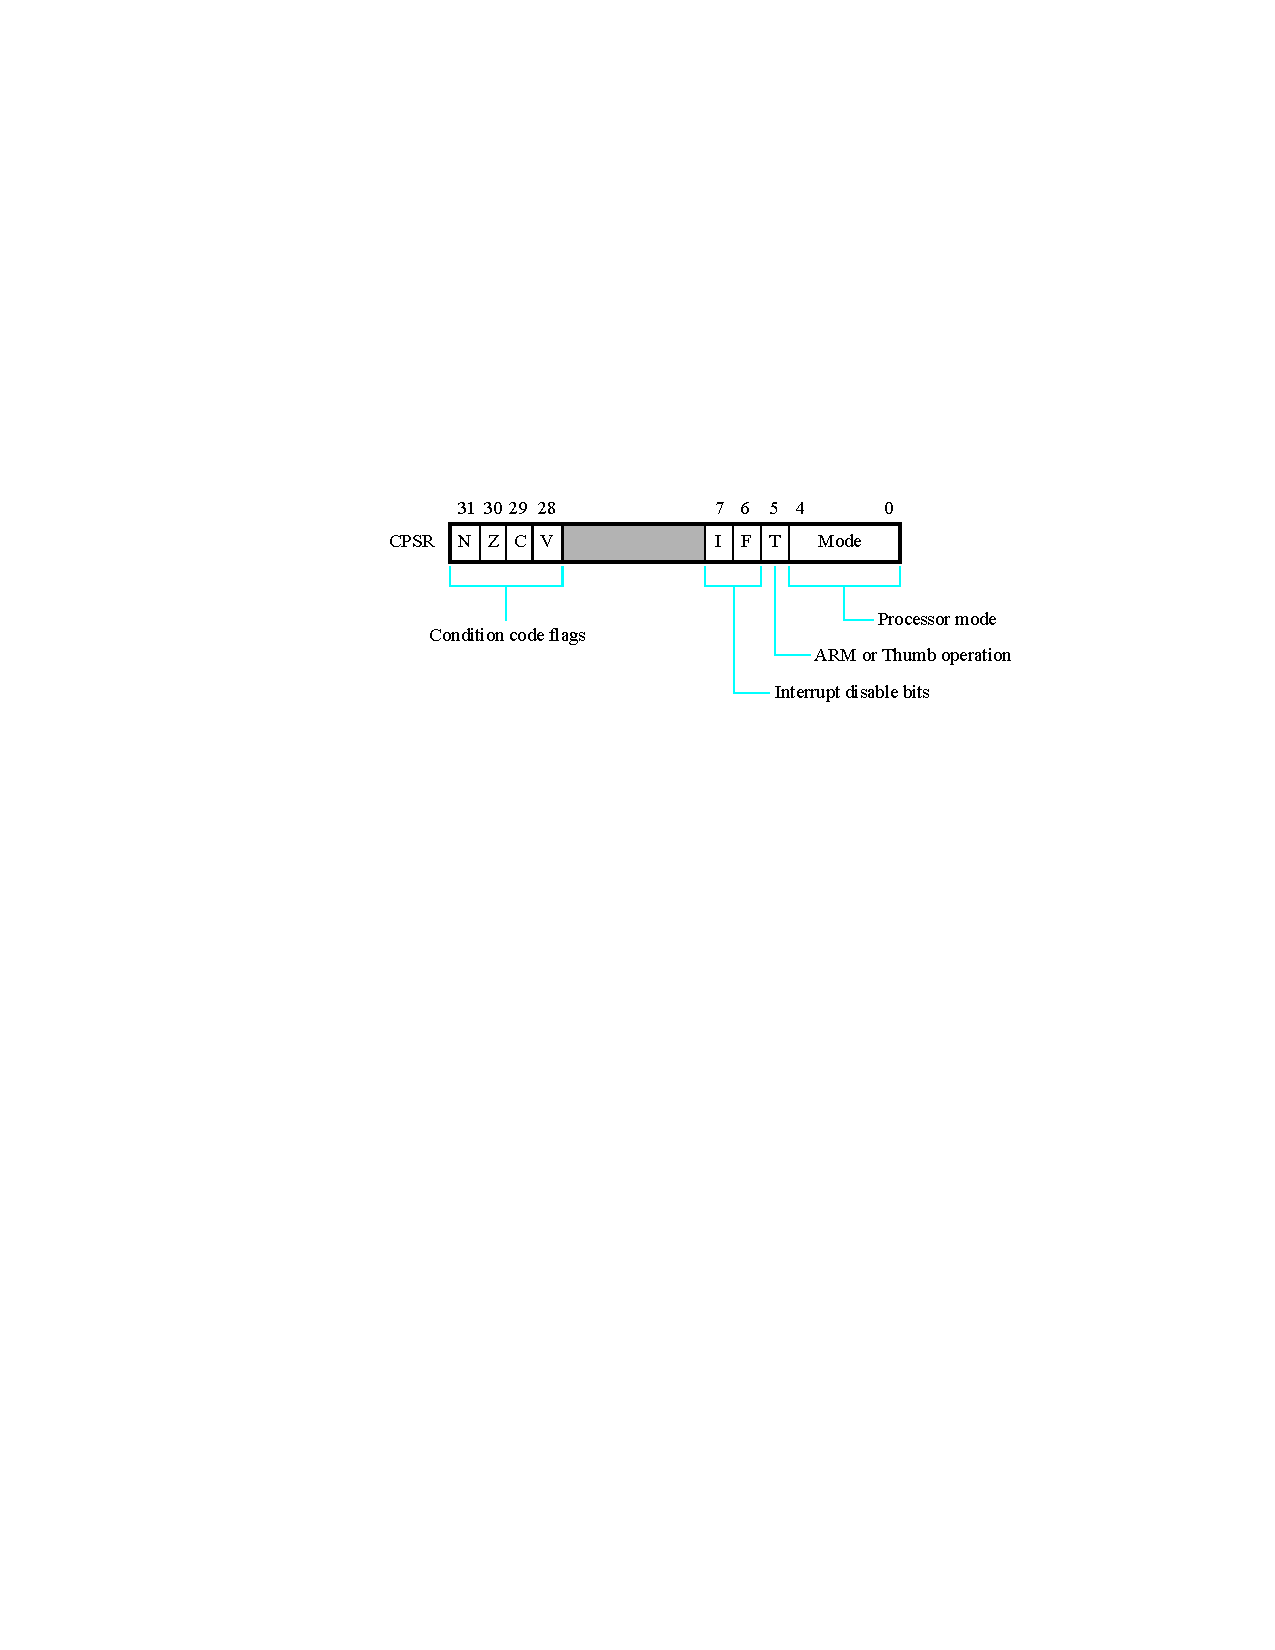
\includegraphics{figures/arm_cpsr.pdf}
   \end{center}
   \caption{The current processor status register (CPSR).}
	\label{fig:arm_cpsr}
\end{figure}

\newcommand{\vs}{\rule{0pt}{1ex}\\}

\begin{center}
{\bf TABLE 1. ~Mode Bits}
\vs
\begin{tabular}{ll}
\hline
\vs
{\bf CPSR$_{4-0}$} & {\bf Operating Mode} \\
\vs
\hline
\vs
10000 & User \\
10001 & FIQ \\
10010 & IRQ \\
10011 & Supervisor \\
10111 & Abort \\
11011 & Undefined \\
11111 & System \\
\vs
\hline
\end{tabular}
\end{center}

To manipulate the contents of the CPSR, the processor must be 
in one of the privileged modes.  Figure~\ref{fig:arm_banked_regs} shows the
general-purpose registers in a Cortex-A9 processor, and illustrates how the registers are
related to the processor mode.  In User mode, there are 16 registers, $R0 - R15$, plus the
CPSR. These registers are also available in the System mode, which is not shown in the
figure. As indicated in Figure~\ref{fig:arm_banked_regs}, $R0 - R12$, as well as the program 
counter $R15$, are common to all modes except FIQ. But the 
stack pointer register $R13$ and the link register $R14$ are not common---{\it banked} 
versions of these registers exist for each mode. Thus, the Supervisor mode has a stack pointer and
link register that are used only when the processor is in this mode. Similarly, the
other modes, such as IRQ mode, have their own stack pointers and 
link registers. The CPSR register is common for all modes, but when the processor is
switched from one mode into another, the current content of the CPSR is copied into the new 
mode's saved processor status register (SPSR). Note that the FIQ mode, which we do not
discuss in this document, has the additional banked registers $R8 - R12$, as shown in the figure.

\begin{figure}[h!]
   \begin{center}
       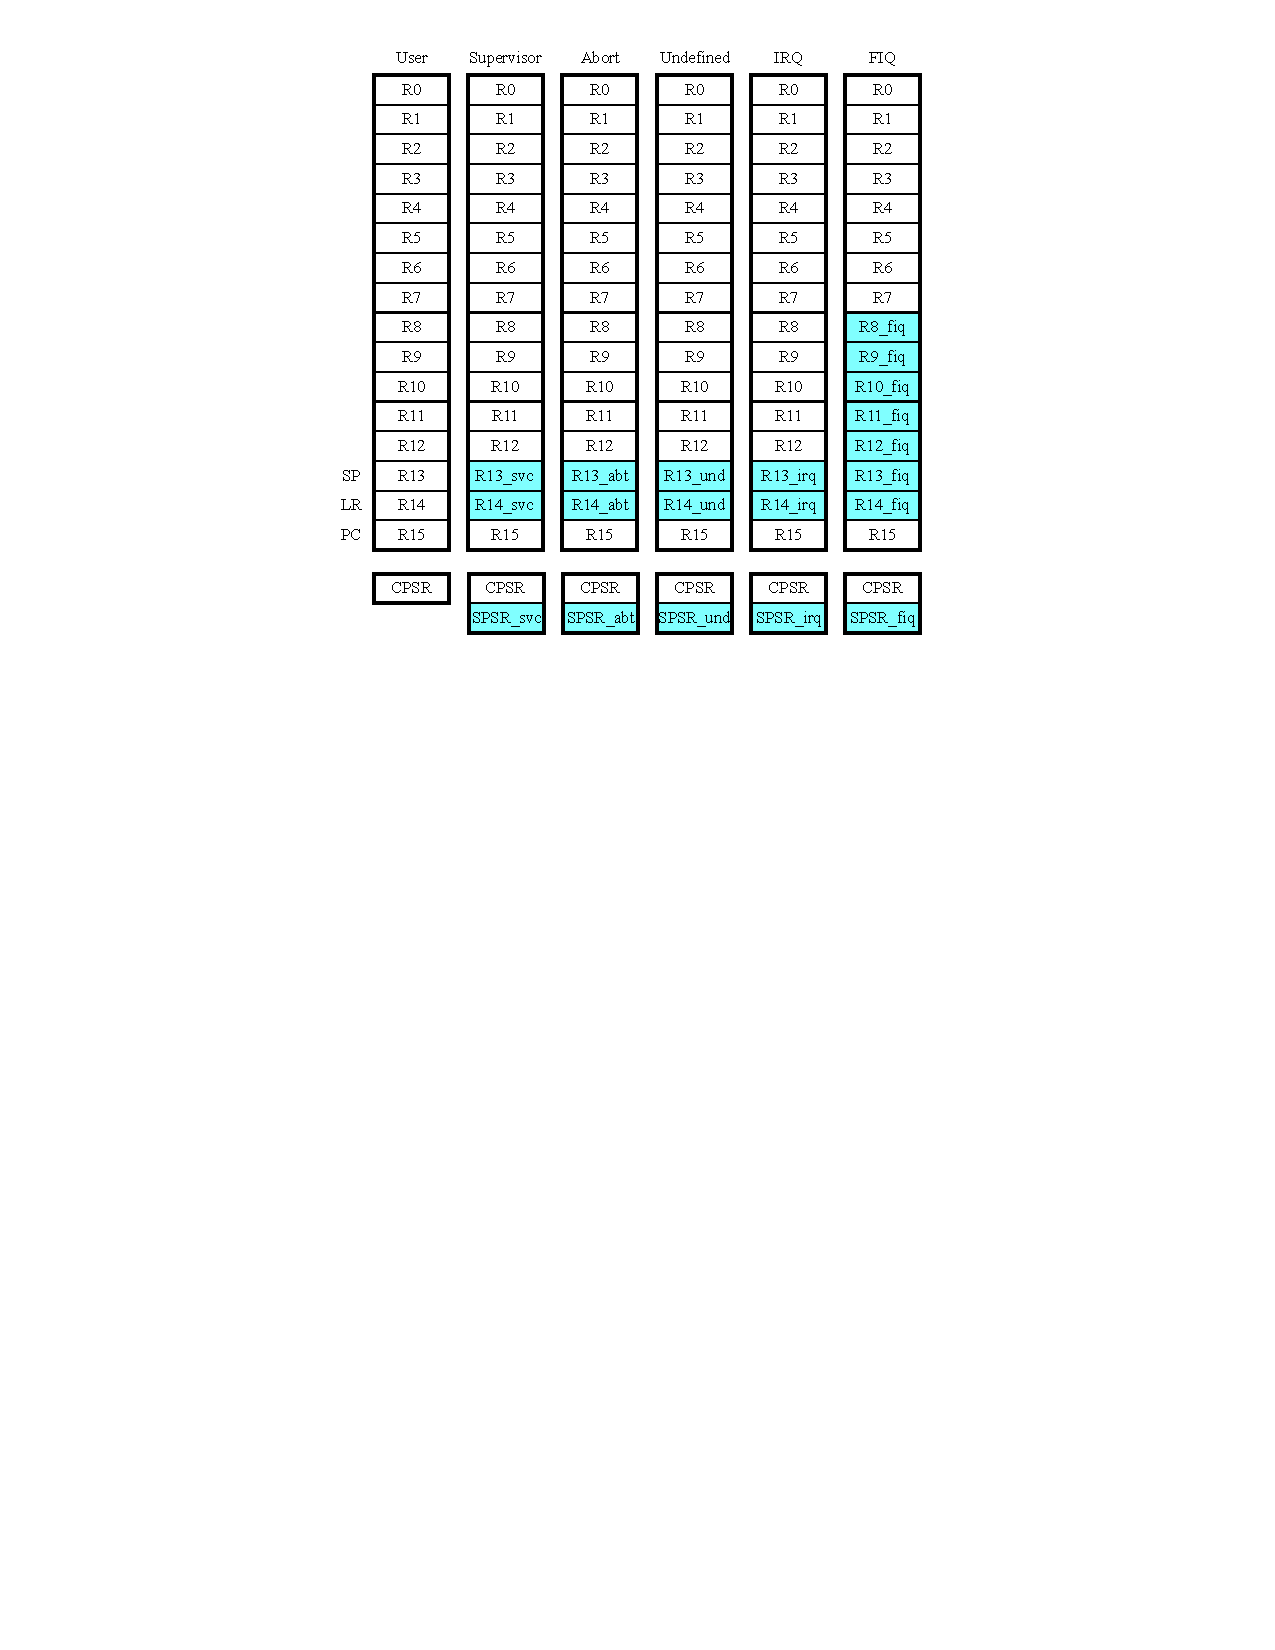
\includegraphics{figures/arm_banked_regs.pdf}
   \end{center}
   \caption{Banked registers in ARM processors.}
	\label{fig:arm_banked_regs}
\end{figure}

\subsection{IRQ Mode}
A Cortex-A9 processor enters IRQ mode in response to receiving an IRQ signal from the GIC.
Before such interrupts can be used, software code has to perform a number of steps:

\begin{enumerate}
	\item Ensure that IRQ interrupts are disabled in the A9 processor, by setting 
			  the IRQ disable bit in the CPSR to 1.
	\item Configure the GIC. Interrupts for each I/O peripheral device that is connected to the GIC 
			  are identified by a unique {\it interrupt~ID}.
	\item Configure each I/O peripheral device so that it can send IRQ interrupt requests to the GIC.
	\item Enable IRQ interrupts in the A9 processor, by setting the IRQ disable bit in the
			  CPSR to 0.
\end{enumerate}

Examples of software code that perform these steps are given in
Sections~\ref{sec:ass_code} and~\ref{sec:C_code}. Complete examples of interrupt-driven
code are included in the appendices.

\section{Programmer's Interface to the GIC}
\label{sec:GIC} The GIC includes a number of memory-mapped registers that provide an
{\it application programmer's interface} (API). As illustrated in Figure~\ref{fig:fig_GIC}, the GIC
architecture is divided into two main parts, called the {\it CPU Interface} and the
{\it Distributor}.  The CPU Interface is responsible for sending IRQ requests received by 
the Distributor to one or both of the A9 processors in the MPCORE.
The Distributor receives IRQ interrupt signals from I/O peripherals.

\begin{figure}[h!]
   \begin{center}
       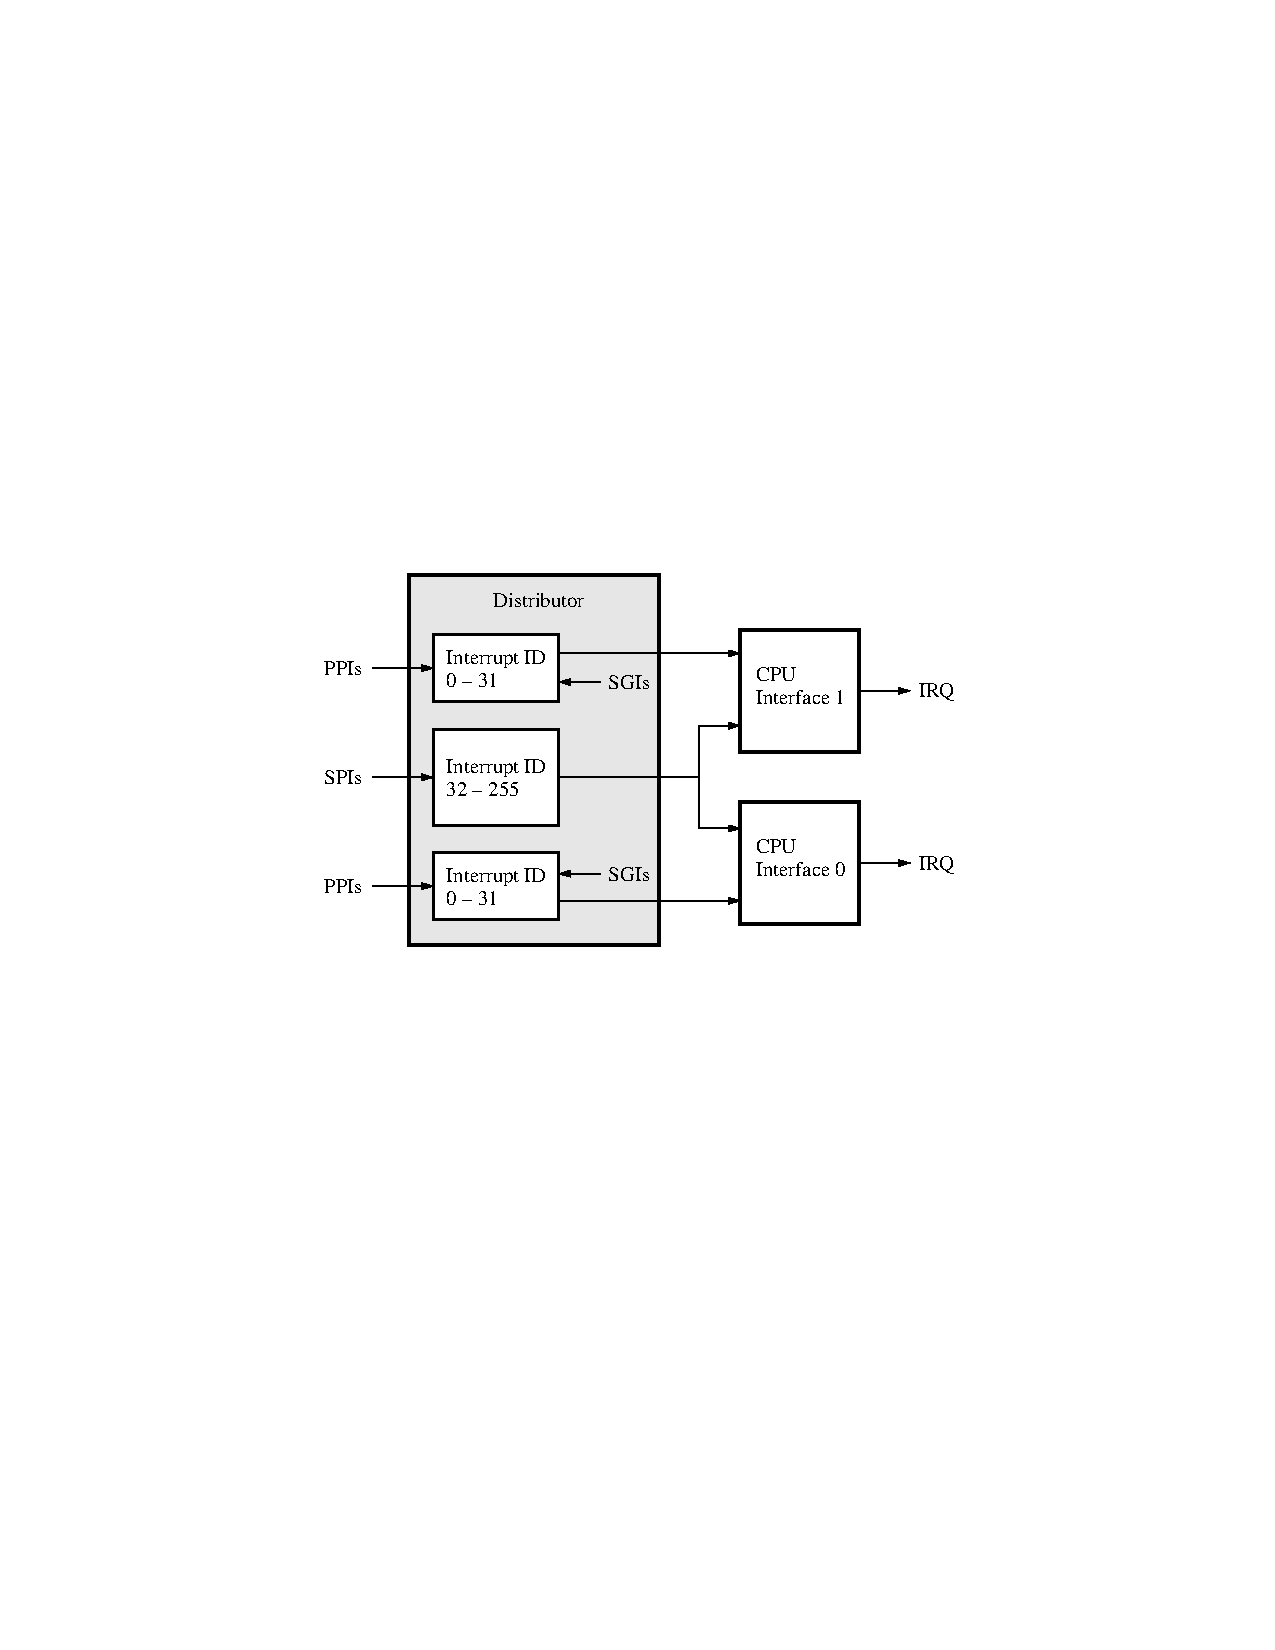
\includegraphics{figures/GIC.pdf}
   \end{center}
   \caption{The GIC Architecture.}
	\label{fig:fig_GIC}
\end{figure}

\subsection{GIC CPU Interface}
\label{sec:CPU_IF} The CPU Interface in the GIC is used to send IRQ signals to the A9
cores. There is one CPU Interface for each A9 core in the MPCORE.  API registers 
in each CPU Interface are depicted in Figure~\ref{fig:CPU_IF}. To make the example more
concrete, we have assigned addresses to these registers, as shown. These addresses
correspond to those used in the document {\it DE1-SoC Computer System with ARM Cortex-A9},
which is available from Intel's FPGA University Program. The DE1-SoC Computer System is an ARM
Cortex-A9 embedded system that can be implemented on Intel's DE1-SoC development and
education board. 

The {\it CPU Interface Control Register} (ICCICR) is used to enable forwarding of
interrupts from the CPU Interface to the corresponding A9 core. 
Setting bit $E=1$ in this register enables the sending
of interrupts to the A9 core, and setting $E=0$ disables these interrupts. 

The {\it Interrupt Priority Mask Register} (ICCPMR) is used to set a threshold for the 
priority-level of interrupts that will be forwarded by a CPU Interface to an A9 core. 
Only interrupts that
have a priority level greater than the {\it Priority} field in ICCPMR will be sent to an
A9 processor by its CPU Interface. Lower priority values represent higher priority,
meaning that level 0 is the highest priority and level 255 is the lowest. Setting the 
{\it Priority} field in ICCPMR to the value 0 will prevent any interrupts from being
generated by the CPU Interface. The procedure for setting the priority level of individual
interrupts (based on their Interrupt ID) is described in Section~\ref{sec:GIC_dist}.

The {\it Interrupt Acknowledge Register} (ICCIAR) contains the Interrupt ID of the
I/O peripheral that has caused an interrupt.  When an A9 processor receives an IRQ
signal from the GIC, software code (i.e., the {\it interrupt handler}) running on the 
processor must read the ICCIAR to determine which I/O peripheral has caused the interrupt. 

After the A9 processor has completed the handling of an IRQ interrupt generated by the
GIC, the processor must then clear this interrupt from the CPU Interface. This action is
accomplished by writing the appropriate Interrupt ID into the {\it Interrupt ID} field in the 
{\it End of Interrupt Register} (ICCEOIR), depicted in Figure~\ref{fig:CPU_IF}.
After writing into the ICCEOIR, the interrupt handler software can then
return control to the previously-interrupted main program.

\begin{figure}[h!]
   \begin{center}
       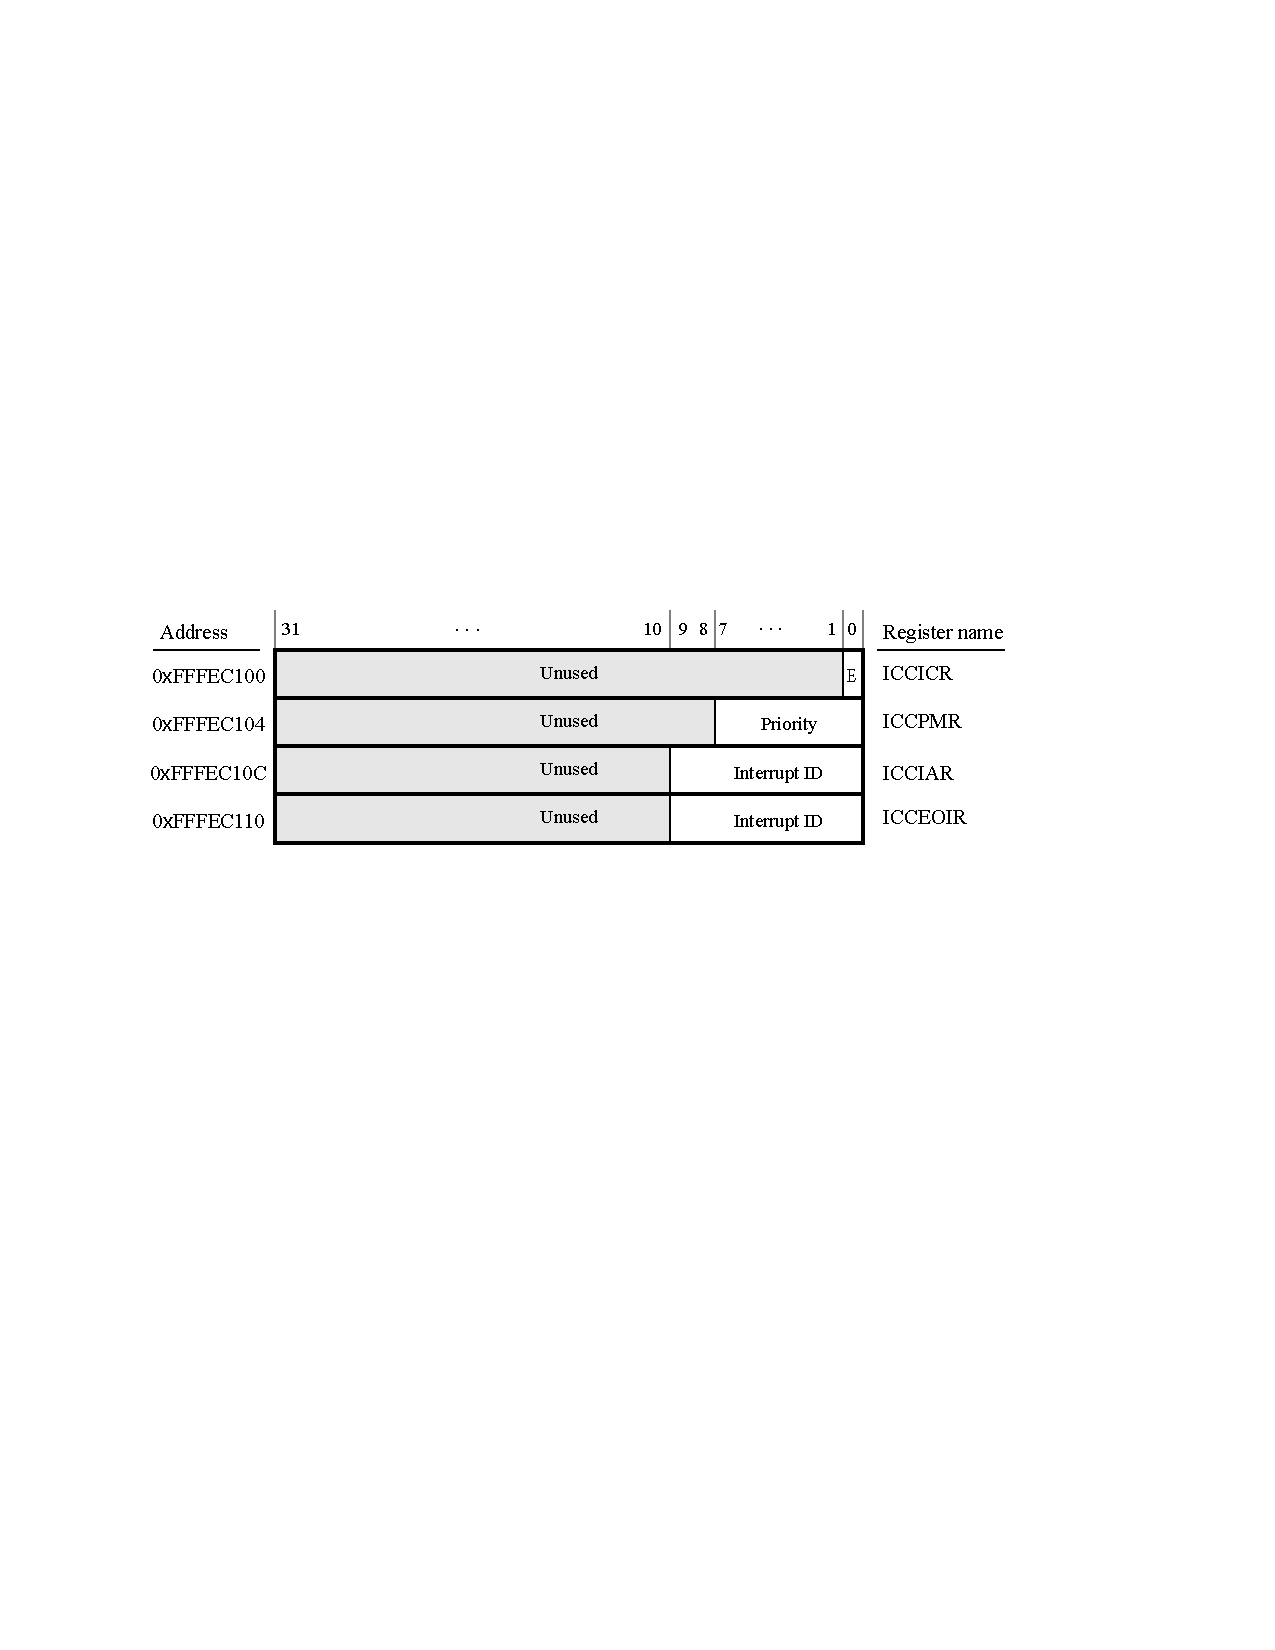
\includegraphics{figures/CPU_IF.pdf}
   \end{center}
   \caption{CPU Interface registers.}
	\label{fig:CPU_IF}
\end{figure}

\subsection{GIC Distributor}
\label{sec:GIC_dist} The Distributor in the GIC can handle 255 sources of interrupts. As
indicated in Figure~\ref{fig:fig_GIC}, Interrupt IDs in the range from $32 - 255$
correspond to {\it shared peripheral interrupts} (SPIs). These interrupts are connected to
the IRQ signals of up to 224 I/O peripherals, and these sources of interrupts are
common to (shared by) both CPU Interfaces. The Distributor also handles {\it private peripherals 
interrupts} (PPIs) for each of the A9 processors, with these interrupts using IDs in the range 
from $0 - 31$. The {\it software generated interrupts} (SGIs) are a special type of
private interrupt that are generated by writing to a specific register in the GIC;
Interrupt IDs from $0 - 15$ are used for SGIs. We do not discuss SGIs further in this
document. 

\begin{figure}[h!]
   \begin{center}
       \includegraphics{figures/distributor.pdf}
   \end{center}
   \caption{Distributor registers.}
	\label{fig:distributor}
\end{figure}

API registers in the Distributor are depicted in Figure~\ref{fig:distributor}. As
described in the previous section, addresses are shown for each register and these addresses 
correspond to those used in the DE1-SoC Computer. The Distributor Control Register
(ICDDCR) is used to enable the Distributor. Setting $E=0$ in this register disables the
Distributor, while setting $E=1$ enables it. 

The {\it Interrupt Set Enable Registers} (ICDISERn) are used to enable the forwarding of 
each supported interrupt from the Distributor to the CPU Interface. The {\it n} postfix in the
name ICDISERn means that multiple registers exist. Referring
to Figure~\ref{fig:distributor}, the set-enable bits for the first 32 Interrupt IDs are
provided in the register at address {\sf 0xFFFED100}, the next 32 are provided in the
register at the following word address, which is {\sf 0xFFFED104}, and so on. Given a
specific Interrupt ID, $N$, the address of the register that contains its set-enable bit is
given by the integer calculation {\it address} $=$ {\sf 0xFFFED100} + $(N \div 32) \times 4$, and 
the index of the bit inside this register is given by {\it index}~$= N \bmod 32$.
Writing the value 1 into a set-enable bit enables the forwarding of the corresponding IRQ 
to the CPU Interface.

In the same way that each supported interrupt can be enabled by using ICDISERn, each 
interrupt can be disabled by using the {\it Interrupt Clear Enable Registers} (ICDICERn). 
The method for calculating the address and index for ICDICERn is the same as that for 
ICDISERn, except that the base address is {\sf 0xFFFED180}, as shown in 
Figure~\ref{fig:distributor}.  Writing a 1 into a clear-enable bit disables the forwarding 
of the corresponding interrupt to the CPU Interface.

The {\it Interrupt Priority Registers} (ICDIPRn) are used to associate a priority level
with each individual interrupt. On reset, these registers are set to {\sf 0x00000000},
which represents the highest priority.  In Figure~\ref{fig:distributor} 
the base address of ICDIPRn is {\sf 0xFFFED400}. Each
Interrupt ID's priority field is one byte in size, which means that the register at the 
base address holds the priority levels for Interrupt IDs from 0 to 3. The
priority levels for the next four Interrupt IDs use the register at address {\sf
0xFFFED404}, and so on.  Given a specific Interrupt ID, $N$, the address of the register 
that contains its priority field is given by the integer calculation 
{\it address}~$=$~{\sf 0xFFFED400}~+~$(N \div 4) \times 4$, and 
the index of the byte inside this register is given by {\it index}~$= N \bmod 4$.
Setting the priority field for an Interrupt ID to a larger number results in lower priority 
for the corresponding interrupt.

The {\it Interrupt Processor Targets Registers} (ICDIPTRn) are used to specify the CPU 
interfaces to which each interrupt should be forwarded. As indicated in 
Figure~\ref{fig:distributor}, the {\it CPUs} field for each Interrupt ID is one byte in
size. This size is used because some versions of the ARM A9 MPCORE have up to eight
A9 cores.  A target CPU is selected by setting its corresponding bit field to 1. Thus,
setting the byte at address {\sf 0xFFFED800} to the value {\sf 0x01} would target Interrupt ID 0
to CPU 0, setting this same byte to {\sf 0x02} would target CPU 1, and setting the byte to the 
value {\sf 0x03} would target both CPU 0 and CPU 1.  The scheme for calculating the address 
of the ICDIPTRn register for a specific Interrupt ID, and also its byte index, is the same 
as the one shown above for ICDIPRn. 

The {\it Interrupt Configuration Registers} (ICDICFRn) are used to specify whether each
supported interrupt should be handled as level- or edge-sensitive by the GIC. As indicated in
Figure~\ref{fig:distributor}, there is a two-bit field associated with each Interrupt ID.
The least-significant bit in this field is not used.  Setting the most-significant bit
of this field to 1 makes the corresponding interrupt signal edge-sensitive, and setting
this field to 0 makes it level-sensitive. When a level-sensitive IRQ signal is asserted by
an I/O peripheral it is possible to de-assert this signal if the interrupt has not yet
been forwarded from the Distributor to a CPU Interface. However, an edge-triggered IRQ 
signal cannot be de-asserted once it has been sampled in the Distributor.
Referring to Figure~\ref{fig:distributor}, the first 16 Interrupt IDs use the ICDICFRn
register at address {\sf 0xFFFEDC00}, the next 16 at address {\sf 0xFFFEDC04}, and so on. 
Given a specific Interrupt ID, $N$, the address of the ICDICFRn register 
is given by the integer calculation 
{\it address}~$=$~{\sf 0xFFFEDC00}~+~$(N \div 16) \times 4$, and 
the index of the bit inside this register is given by {\it index}~$= (N \bmod 16)+1$.

\newpage
\section{Example of Assembly Language Code}
\label{sec:ass_code}Figure \ref{fig:ass_code} provides an example of an assembly language
subroutine that configures the GIC. This code configures Interrupt ID~73, as an example, which
corresponds to a parallel port connected to pushbutton KEYs in the DE1-SoC Computer. The code
configures only some of the registers in the GIC and uses acceptable default values for
other registers. A complete example of code that uses this subroutine is provided in the
Appendix A.

\begin{figure}[h!]
\begin{center}
\lstinputlisting[style=defaultArmStyle, lastline=31]{design_files/config_GIC.s}
\end{center}
\caption{An example of assembly language code that configures the GIC (Part $a$).}
   \label{fig:ass_code}
\end{figure}

\clearpage
\begin{center}
\lstinputlisting[style=defaultArmStyle, firstline=32]{design_files/config_GIC.s}
Figure \ref{fig:ass_code}. An example of assembly language code that configures the GIC (Part $b$).
\end{center}

\newpage
\section{Example of C Code}
\label{sec:C_code} Figure \ref{fig:C_code} provides an example of a subroutine written in
C code that configures the GIC. This code performs the same operations as the assembly
language code shown in Figure~\ref{fig:ass_code}.  A complete program that uses 
this subroutine is provided in the Appendix B.

\begin{figure}[h!]
\begin{center}
\lstinputlisting[language=C, firstline=82, lastline=117]{design_files/exceptions.c}
\end{center}
\caption{An example of C language code that configures the GIC (Part $a$).}
   \label{fig:C_code}
\end{figure}

\clearpage
\begin{center}
\lstinputlisting[language=C, firstline=119]{design_files/exceptions.c}
\end{center}
\begin{center}
Figure \ref{fig:C_code}. An example of C code that configures the GIC (Part $b$).
\end{center}

\newpage
\appendix{\LARGE{\bf {Appendix A: Example Assembly Language Program}}}

\lstinputlisting[style=defaultArmStyle]{design_files/interrupt_example.s}
\lstinputlisting[style=defaultArmStyle]{design_files/config_GIC.s}
\lstinputlisting[style=defaultArmStyle]{design_files/key_isr.s}

\newpage
\appendix{\LARGE{\bf {Appendix B: Example C Program}}}

\lstinputlisting[language=C]{design_files/interrupt_example.c}
\lstinputlisting[language=C]{design_files/exceptions.c}
\lstinputlisting[language=C]{design_files/pushbutton_ISR.c}

% Copyright and Trademark

%\newcommand{\datePublished}{Mar 2022}

\newcommand{\versnum}{21.1} %version number quartus/AMP
\newcommand{\quartusname}{Quartus\textsuperscript{\textregistered} Prime}	
\newcommand{\textBar}{For \quartusname{} \versnum{}}
\newcommand{\thisyear}{2022 } %for copyright
\newcommand{\company}{FPGAcademy.org}
\newcommand{\longteamname}{FPGAcademy.org}
\newcommand{\teamname}{FPGAcademy}
\newcommand{\website}{FPGAcademy.org}

\newcommand{\productAcronym}{AMP}
\newcommand{\productNameShort}{Monitor Program}

\newcommand{\productNameMedTM}{Monitor Program}
\newcommand{\productNameMed}{Monitor Program}

%\newcommand{\headerLogoFilePath}[1]{#1/FPGAcademy.png}



%%%%%%%%%%%%%%%%%%%%%%%%%%%%%%%%%%%%%%%%
%%% FPGAcademy Copyright Information %%%
%%%%%%%%%%%%%%%%%%%%%%%%%%%%%%%%%%%%%%%%

%Always put the copyright on a new page (clear page), with some vertical space from top
\clearpage
\vspace{1in}

\noindent

Copyright {\copyright} FPGAcademy.org. All rights reserved. FPGAcademy and the FPGAcademy logo are trademarks of  FPGAcademy.org.  This document is being provided on an ``as-is'' basis and as an accommodation and therefore all warranties, representations or guarantees of any kind (whether express, implied or statutory) including, without limitation, warranties of merchantability, non-infringement, or fitness for a particular purpose, are specifically disclaimed.

%FPGAcademy assumes no responsibility or liability arising out of the application or use of any information,  product,  or  service  described  herein  except  as  expressly  agreed  to  in  writing  by  FPGAcademy.



**Other names and brands may be claimed as the property of others.




\end{document}
